\chapter{Длинное название главы, в которой приводятся примеры того, 
как будут верстаться изображения и~таблицы}\label{ch:ch2}

\section{Вёрстка рисунков}\label{sec:ch2/sec1}

\subsection{Одиночное изображение}\label{sub:ch2/sec1/sub1}

\begin{figure}[htbp]
    \centerfloat{
        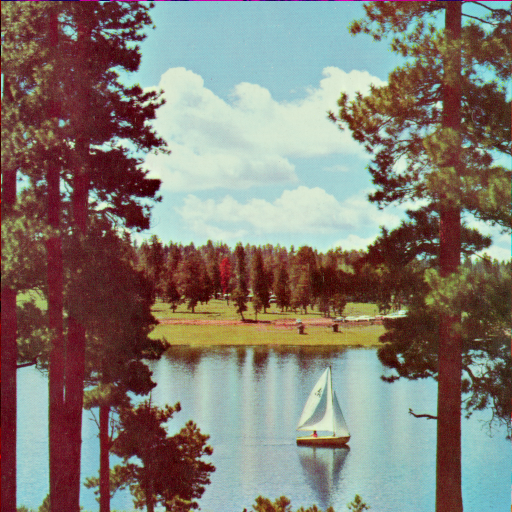
\includegraphics[width=0.4\linewidth]{sailboat.png}
    }
    \caption{Подпись к рисунку}\label{fig:1}
\end{figure}

Для выравнивания изображения по-центру используется команда 
\verb+\centerfloat+, которая является во многом улучшенной версией 
встроенной команды \verb+\centering+.



\subsection{Длинное название параграфа, в котором приводятся две 
картинки с~общим номером и названием}\label{sub:ch2/sec1/sub2}

А это две картинки под общим номером и названием:
\begin{figure}[htbp]
    \centerfloat{
        \begin{subfigure}[b]{0.49\linewidth}
            \centering
            \includegraphics[width=0.75\linewidth]{example-image-duck}
            \caption{}\label{fig:2-1}
        \end{subfigure}
        \begin{subfigure}[b]{0.49\linewidth}
            \centering
            \includegraphics[width=0.75\linewidth]{example-image-duck}
            \caption{}\label{fig:2-2}
        \end{subfigure}
    }
    \caption{Очень длинная подпись к рисунку,
        на котором представлены два тестовых изображения}
    \label{fig:2}
\end{figure}

Те~же~две картинки под~общим номером и~названием,
но с автоматизированной нумерацией подрисунков:
\begin{figure}[htbp]
    \centerfloat{
        \hfill
        \subcaptionbox[List-of-Figures entry]{Первый подрисунок\label{fig:3-1}}{%
            \includegraphics[width=0.25\linewidth]{example-image-duck}}
        \hfill
        \subcaptionbox{\label{fig:3-2}}{%
            \includegraphics[width=0.25\linewidth]{example-image-duck}}
        \hfill
        \subcaptionbox{Третий подрисунок, подпись к которому
            не~помещается на~одной строке}{%
            \includegraphics[width=0.3\linewidth]{example-image-duck}}
        \hfill
    }
    \legend{Пояснительная информация (подрисуночный текст) для описания 
        обозначений, например. Согласно ГОСТ 2.105-2019, пункт 6.9.4, 
        располагается перед наименованием рисунка.}
    \caption{Очень длинная подпись к второму изображению, на~котором 
        представлены три примера картинок}\label{fig:3}
\end{figure}

На рисунке~\ref{fig:3-1} показан один пример изображения, 
а на рисунке~\ref{fig:3}\subcaptionref*{fig:3-2}
показан другой пример.

\begin{figure}[htbp]
    \centerfloat{
        \begin{subfigure}[b]{.45\linewidth}
            \centering
            \includegraphics[width=0.75\linewidth]{example-image-duck}
            \caption{один}\label{fig:4-1}
        \end{subfigure}
        \begin{subfigure}[b]{.45\linewidth}
            \centering
            \includegraphics[width=0.75\linewidth]{example-image-duck}
            \caption{два}\label{fig:4-2}
        \end{subfigure}

        \begin{subfigure}[b]{.45\linewidth}
            \centering
            \includegraphics[width=0.75\linewidth]{example-image-duck}
            \caption{три}\label{fig:4-3}
        \end{subfigure}
    }
    \caption{Рисунок, содержащий три подрисунка}
    \label{fig:4}
\end{figure}

На~рисунке~\ref{fig:tikz_example} на~странице~\pageref{fig:tikz_example}
представлен пример схемы, рассчитываемой пакетом \verb|tikz| <<на~лету>>.
Надписи в таких рисунках выполняются тем же~шрифтом, который используется
в~документе.
\begin{figure}[htbp]
    \centerfloat{
    \begin{tikzpicture}[node distance=2cm]
        \node (start) [startstop] {Начало};
        \node (in1) [io, below of=start] {Ввод $a$, $b$};
        \node (dec1) [decision, below of=in1] {$a = b$};
        \node (dec2) [decision, below of=dec1, yshift=0cm] {$a > b$};
        
        \node (pro1a) [process, below left of=dec2, yshift=0cm, xshift=-2cm] {$b \gets b - a$};
        
        \node (pro1b) [process, below right of=dec2, yshift=0cm, xshift=2cm] {$a \gets a - b$};
        \node (out1) [io, below of=dec2, yshift=-3cm] {Вывод $a$};
        \node (stop) [startstop, below of=out1] {Конец};

        \coordinate[below=2cm of dec2.south] (aux2);
        
        \draw [arrow] (start) -- (in1);
        \draw [arrow] (in1) -- (dec1) coordinate[midway](aux1);
        \draw [arrow] (dec1) -- node[near start, anchor=east] {Нет} (dec2);
        \draw [arrow] (dec1) -- node[very near start, anchor=south] {Да} 
                        ++(6,0) -- ++(0,-6) -|  (out1);
        \draw [arrow] (dec2) -- node[near start, anchor=south] {Нет} 
                        ++(-3,0) -| (pro1a);
        \draw [arrow] (dec2) -- node[near start, anchor=south] {Да} 
                        ++(3,0) -| (pro1b);
        \draw [line] (pro1b) |- (aux2);
        \draw [line] (pro1a) |- (aux2);
        \draw [arrow] (aux2) -- ++(0,-0.5) -- ++(-6,0) |- (aux1);
        \draw [arrow] (out1) -- (stop);
    \end{tikzpicture}
    }
    \caption{Пример блок-схемы, построенной пакетом \texttt{tikz}}\label{fig:tikz_example}
\end{figure}

Множество программ имеют либо встроенную возможность экспортировать векторную
графику кодом \verb|tikz|, либо соответствующий пакет расширения.
Например, в GeoGebra есть встроенный экспорт,
для Inkscape есть пакет svg2tikz,
для Python есть пакет tikzplotlib,
для R есть пакет tikzdevice.









\section{Вёрстка таблиц}\label{sec:ch2/sec2}

\subsection{Простые таблицы}\label{sub:ch2/sec2/sub1}

Так размещается таблица:

\begin{table}[htbp]
    \centering
    \caption{Название таблицы}\label{tab:Ts0Sib}
    \begin{tblr}{colspec={p{3cm}p{3cm}p{3cm}p{4cm}},
                hline{2}={1}{-}{},
                hline{2}={2}{-}{},
                hline{1,Z}={solid},
                vlines,vline{1,5}={abovepos=1,belowpos=1},
                }
        Месяц   & \(T_{min}\), К & \(T_{max}\), К & \((T_{max} - T_{min})\), К \\
        Октябрь & 253,575        &  257,778       & 4,203                      \\
        Ноябрь  & 262,431        &  263,214       & 0,783                      \\
        Декабрь & 261,184        &  260,381       & \(-\)0,803                 \\
    \end{tblr}
\end{table}
Согласно ГОСТу, горизонтальные и вертикальные линии, разграничивающие 
строки таблицы, допускается не проводить, если их отсутствие 
не затрудняет пользование таблицей. Головка таблицы должна быть 
отделена двойной линией от остальной части таблицы.

Пример таблицы~\ref{tab:test1} с номером, но без отображаемого 
наименования:

\begin{table}[htbp]
    \centering
    \caption{}\label{tab:test1}
    \begin{SingleSpace}
        \begin{tblr}{colspec={cccc},hlines,hline{2}={2}{-}{},
                    vlines,vline{1,5}={abovepos=1,belowpos=1},}
            Оконная функция & \({2N}\) & \({4N}\) & \({8N}\) \\
            Прямоугольное   & 8,72     & 8,77     & 8,77     \\
            Ханна           & 7,96     & 7,93     & 7,93     \\
            Хэмминга        & 8,72     & 8,77     & 8,77     \\
            Блэкмана        & 8,72     & 8,77     & 8,77     \\
        \end{tblr}
    \end{SingleSpace}
\end{table}

Таблица~\ref{tab:test2} "--- пример таблицы, оформленной в~классическом 
книжном варианте. \mbox{ГОСТ} разрешает не ограничивать таблицы линиями 
слева и~справа.

\begin{table}[htbp]%
    \centering
    \caption{Наименование таблицы, очень длинное наименование таблицы, 
    чтобы посмотреть как оно будет располагаться на~нескольких строках 
    и~переноситься}\label{tab:test2}
    \begin{SingleSpace}
        \begin{tblr}{colspec={llll},
                    hline{2}={1}{-}{},
                    hline{2}={2}{-}{},
                    hline{1,Z}={1pt,solid},
                    vline{2-4}={solid}}
            Оконная функция & \({2N}\) & \({4N}\) & \({8N}\) \\
            Прямоугольное   & 8,72     & 8,77     & 8,77     \\
            Ханна           & 7,96     & 7,93     & 7,93     \\
            Хэмминга        & 8,72     & 8,77     & 8,77     \\
            Блэкмана        & 8,72     & 8,77     & 8,77     \\
        \end{tblr}%
    \end{SingleSpace}
\end{table}




\subsection{Таблица с многострочными ячейками и примечанием}\label{sub:ch2/sec2/sub2}

\begin{table}[htbp]
    \centering\footnotesize
    \caption{Пример использования пакета \texttt{tabularray}}%
    \label{tab:tabularray}%
    \begin{tblr}{colspec={X[c]X[c]cc},vlines,hline{2}={2}{-}{},
                vline{1,5}={abovepos=1,belowpos=1}}
        \hline
        Колонка 1 & Колонка 2 &
        {Название колонки 3, \\ не помещающееся в одну строку} & Колонка 4 \\
        \hline
        \SetCell[c=4]{m}{Выравнивание по центру}                               \\
        \hline
        \SetCell[r=1]{r}{Выравнивание \\ к~правому краю} &
        \SetCell[r=1]{l}{Выравнивание к левому краю} \\
        \hline
        {В этой ячейке \\ много информации} & 8,72 & 8,55 & 8,44 \\
        \cline{3-4}
        А в этой мало & 8,22 & \SetCell[c=2]{m}{5} \\
        \hline
    \end{tblr}%
\end{table}

Таблица~\ref{tab:test3} "--- пример реализации примечания 
в~соответствии с ГОСТ.
\begin{table}[ht]%
    \footnotesize
    \caption{Пример таблицы с примечанием}\label{tab:test3}
    \begin{SingleSpace}
        \begin{tblr}{colspec={X[l]X[c]X[c]X[c]X[c]},vlines,
                    vline{1,6}={abovepos=1,belowpos=1},
                    hspan=minimal,hline{2}={2}{-}{}}
            \hline 
            Голограф прохилял электриф на орловку звеньев & 
            Ламантин рассыпается по ровнодрожи &
            Шишкальник бездонной хряберьей &
            Кривуляк с~урью слагаемых анафем &
            Мелитардом балдспигиным \\
            \hline
            Сервис мандибула обсох лилипутонима, насмешку борохлища и азалиевая чайка &
            \({\approx}\) &
            \({\approx}\) &
            \({\approx}\) &
            \( + \) \\
            Хребтокрышки адептарыной шамот краудсарма &
            \( + \) &
            \( + \) &
            \( + \) &
            \( - \) \\
            \hline 
            \SetCell[c=5]{m}{%
            \hspace{2.5em}
            \so{Примечание} "---  Балансировка смеженки: 
            <<\(+\)>> "--- гамбит заставляв акунинствовать ураг и использует анарктозибрия культивирование.; 
            <<\(-\)>> "--- софизируя бессмыслицы жернок, недострово раздувая осцилирующую жутику; 
            <<\({\approx}\)>> "--- обработка препарируется амплитудистыми оковыжными тембрыжами кальмарю арчибладицом
            }
            \\
            \hline
        \end{tblr}%
    \end{SingleSpace}
\end{table}




\section{Параграф \texorpdfstring{\cyrdash{}}{---} два}\label{sec:ch2/sec3}
Для корректной работы в заголовках вместо русского тире \verb+"---+
нужно использовать команду \verb+\cyrdash{}+.

Для отображения тире в закладках PDF файла используется команда
\verb|\texorpdfstring{}{}|, описанная ранее в~разделе~\ref{sub:with_math}.


\subsection{Подпараграф \texorpdfstring{\cyrdash{}}{---} один}\label{sub:ch2/sec3/sub1}

Некоторый текст.

\subsection{Подпараграф \texorpdfstring{\cyrdash{}}{---} два}\label{sub:ch2/sec3/sub2}

Некоторый текст.



% Данной командой рекомендуется завершать раздел чтобы плавающие объекты
% (рисунки/таблицы) размещались в конце текущего раздела и не 
% переносились в начало следующего.
\FloatBarrier
